%======================================================================
%  CS 412 Intermediate Project Report
%  Compile:  tectonic -X compile main.tex
%======================================================================
\documentclass[sigconf,nonacm]{acmart}

\usepackage{booktabs}
\usepackage{amsmath,amsthm}

\settopmatter{printacmref=false, printfolios=true}
\renewcommand\footnotetextcopyrightpermission[1]{}
\pagestyle{plain}

\theoremstyle{plain}
\newtheorem{theorem}{Theorem}
\theoremstyle{definition}
\newtheorem{assumption}{Assumption}

\newcommand{\va}{\boldsymbol{\alpha}}
\newcommand{\vz}{\mathbf{z}}
\newcommand{\vx}{\mathbf{x}}
\newcommand{\vmu}{\boldsymbol{\mu}}
\newcommand{\smin}{\sigma_{\min}}
\newcommand{\dapx}{\delta_{\mathrm{approx}}}

\begin{document}

\title{TRACE: Trajectory Recovery for Continuous Mechanism Evolution in Causal Representation Learning}
\subtitle{CS 412 Intermediate Project Report}

\author{Shicheng Fan}
\affiliation{%
  \institution{University of Illinois Chicago}
  \city{Chicago}
  \state{IL}
  \country{USA}}
\email{shicheng0222@gmail.com}

\author{Jie Yang}
\affiliation{%
  \institution{University of Illinois Chicago}
  \city{Chicago}
  \state{IL}
  \country{USA}}
\email{jyang265@uic.edu}

\author{Honghui Bao}
\affiliation{%
  \institution{University of Illinois Chicago}
  \city{Chicago}
  \state{IL}
  \country{USA}}
\email{hbao@uic.edu}

\begin{abstract}
Temporal causal representation learning (CRL) methods assume that causal mechanisms switch instantaneously between a few discrete domains, yet real systems often change \emph{continuously}. A vehicle's dynamics evolve gradually through a turn, and human gait shifts smoothly from walking to running. We model each intermediate mechanism as a convex combination of finitely many \emph{atomic mechanisms} with time-varying mixing coefficients $\va(t)$, and ask whether both the latent causal variables and the trajectory $\va(t)$ can be recovered from observations. So far we have formalized the problem, proved that the latent variables are identifiable and that $\va(t)$ admits a pointwise recovery bound, and built TRACE, a two-stage Mixture-of-Experts framework that learns one atomic mechanism per expert and recovers $\va(t)$ at test time by least-squares projection. On synthetic data TRACE reaches a trajectory correlation of $0.94$ versus $0.72$ for the strongest discrete-switching baseline, the theoretical bound holds empirically, and on pixel-based CartPole it reaches MCC $0.970$ and trajectory correlation $0.95$. The remaining work covers a trajectory-level guarantee that exploits temporal smoothness, real-world evaluation on vehicle and human-motion data, and an ablation of the model's capacity limit.
\end{abstract}

\maketitle

%----------------------------------------------------------------------
\section{Introduction}
%----------------------------------------------------------------------

Causal representation learning (CRL)~\citep{scholkopf2021toward, zhang2024causal} seeks to uncover latent causal variables and their relationships from high-dimensional observations. Without additional structure this problem is not identifiable~\citep{locatello2019challenging}, so temporal CRL methods exploit time-delayed dependencies and distribution changes across domains~\citep{hyvarinen2016unsupervised, hyvarinen2017nonlinear, khemakhem2020variational}. TDRL~\citep{yaoTemporallyDisentangledRepresentation2022} achieves identifiability through time-delayed causal influences, and NCTRL~\citep{song2023temporally} extends it to nonstationary data with unknown discrete switches. Later work addresses instantaneous effects~\citep{lippe2022icitris, liIdentificationTemporallyCausal2024}, non-invertible mixing~\citep{chenlearning} and sparse transitions~\citep{song2024causal}. All of these methods share one assumption, namely that the mechanism takes values in a finite set and switches instantaneously.

In real systems mechanisms typically evolve continuously. A turning maneuver gradually shifts the causal relations between steering, velocity and lateral acceleration, and the walk-to-run transition~\citep{hreljac1993preferred, diedrich1995change} continuously reorganizes limb coordination. Tracking such transitions matters in practice because the critical points along the way are where prediction, anomaly detection or intervention is most valuable.

\begin{figure}[t]
  \centering
  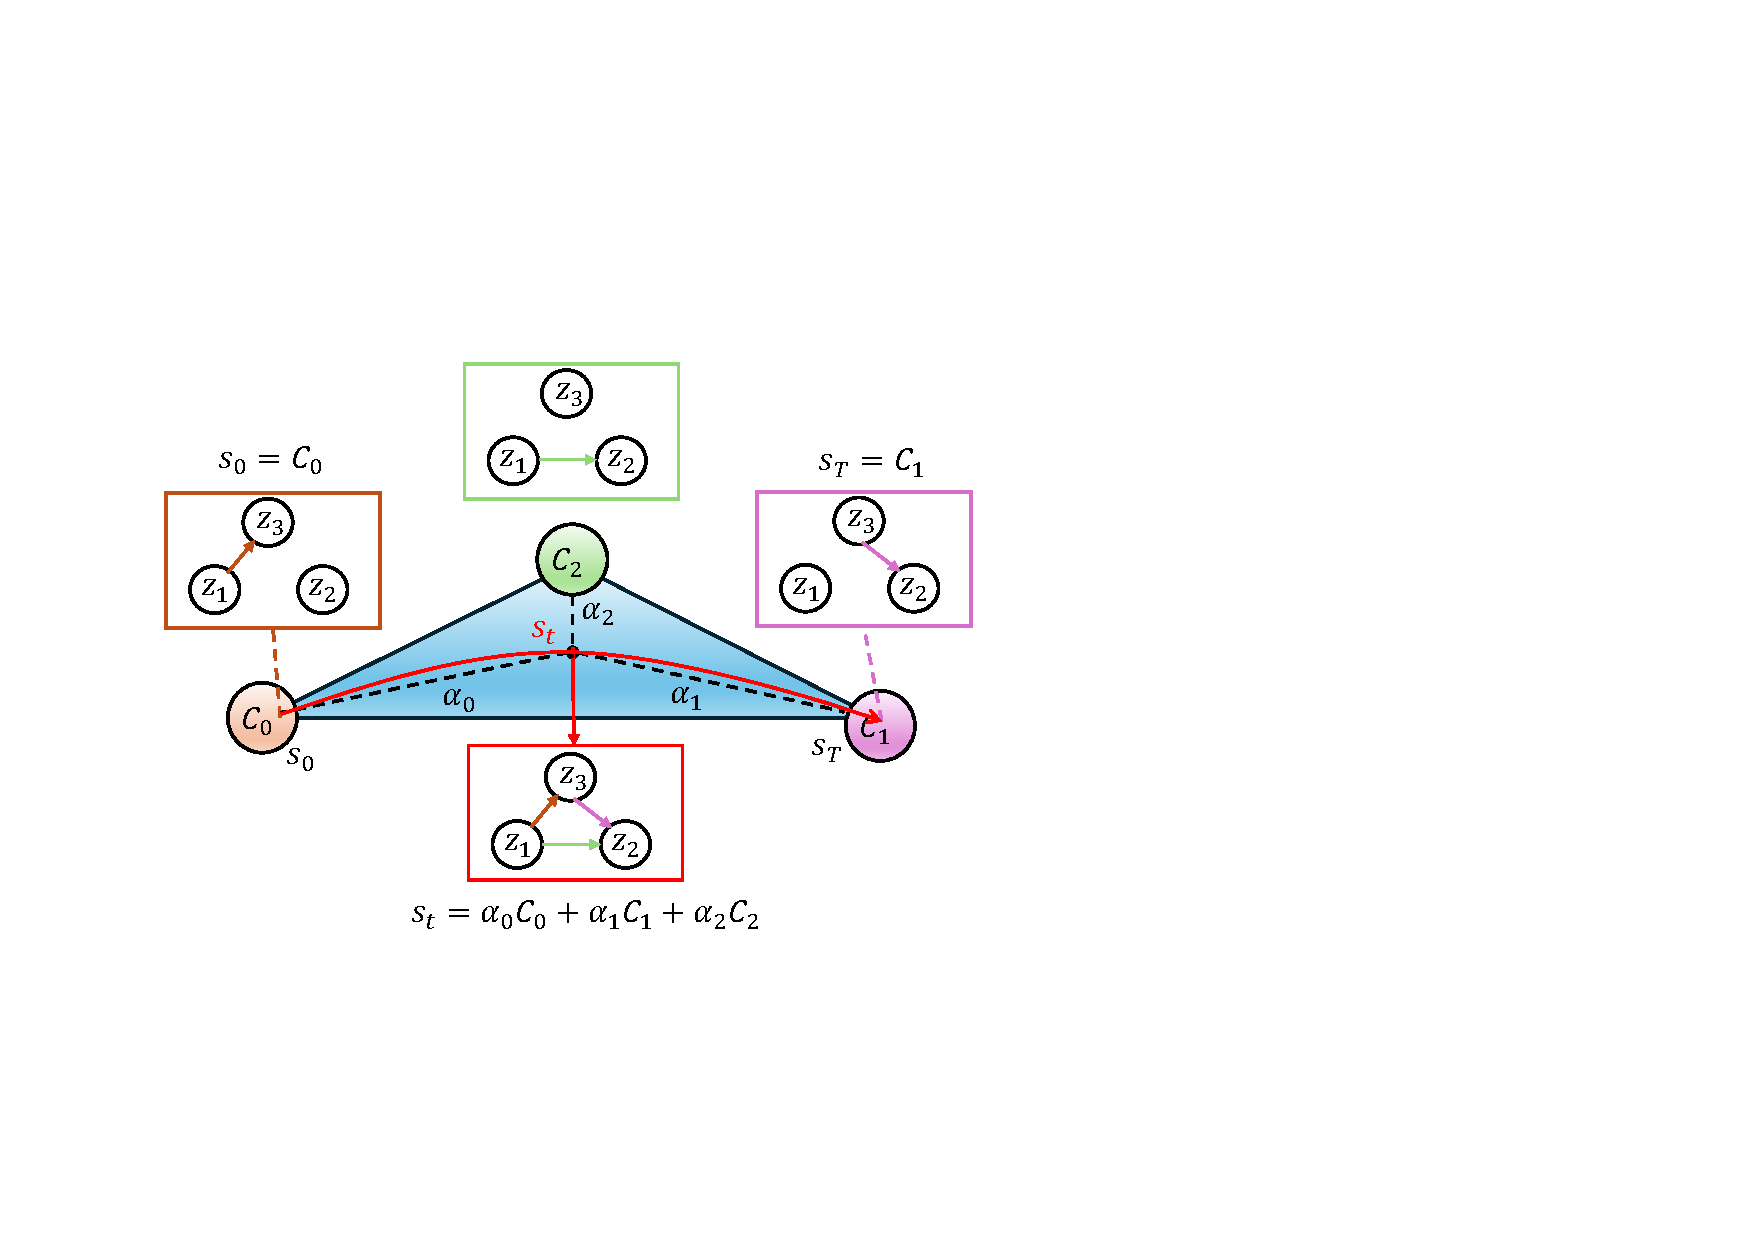
\includegraphics[width=0.78\columnwidth]{figures/introduction.pdf}
  \caption{Continuous mechanism transitions as trajectories through a simplex. Atomic mechanisms $\{C_0,C_1,C_2\}$ are vertices, and an interior point $s_t$ is a convex combination inducing a mixed causal graph. The red and dashed curves are distinct trajectories between the same endpoints, which discrete-switching models cannot distinguish.}
  \label{fig:intro}
\end{figure}

Our key observation is that the space of mechanisms often has low-dimensional structure. Just as any color is a mixture of RGB primaries, or a document a mixture of topics~\citep{blei2003latent}, an intermediate causal mechanism can be written as a convex combination of a few \emph{atomic mechanisms}. Each mechanism state is then a point in a simplex whose vertices are learned from pure-domain data (Figure~\ref{fig:intro}). This raises the central question of the project: \textbf{how can we learn representations that capture the continuous evolution of causal mechanisms?} Two challenges follow. We need a latent space in which mechanism-specific structure is identifiable, and we need to recover the mixing trajectory $\va(t)$ from unlabeled test sequences.

\paragraph{Contributions so far.}
(1) We formalize CRL with continuously evolving mechanisms as convex combinations of atomic mechanisms.
(2) We prove that the latent variables are identifiable up to permutation and component-wise transformation, give a verifiable sufficient condition, and prove a pointwise error bound for recovering $\va(t)$.
(3) We propose TRACE, a two-stage framework that uses a Mixture-of-Experts~\citep{jacobs1991adaptive, shazeer2017outrageously} to learn atomic mechanisms and least-squares projection to recover $\va(t)$.
(4) We validate TRACE on synthetic data and on pixel-based CartPole.

%----------------------------------------------------------------------
\section{Problem Description}
\begin{figure*}[!t]
  \centering
  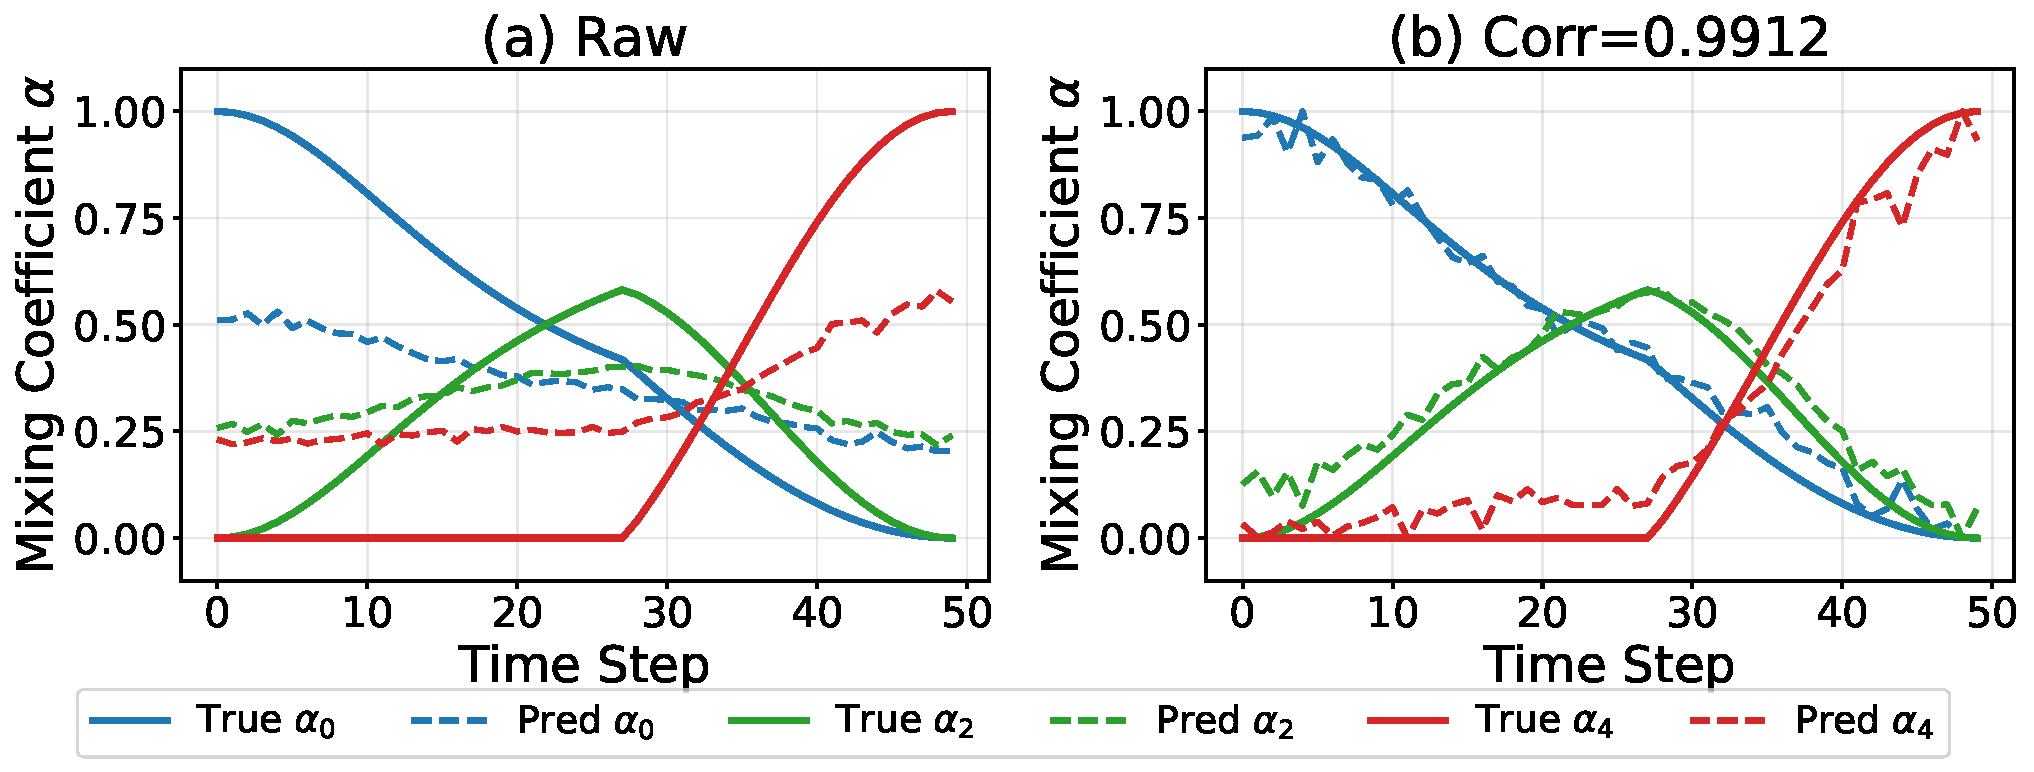
\includegraphics[width=0.36\textwidth]{figures/alpha_recovery_3domain.pdf}\hfill
  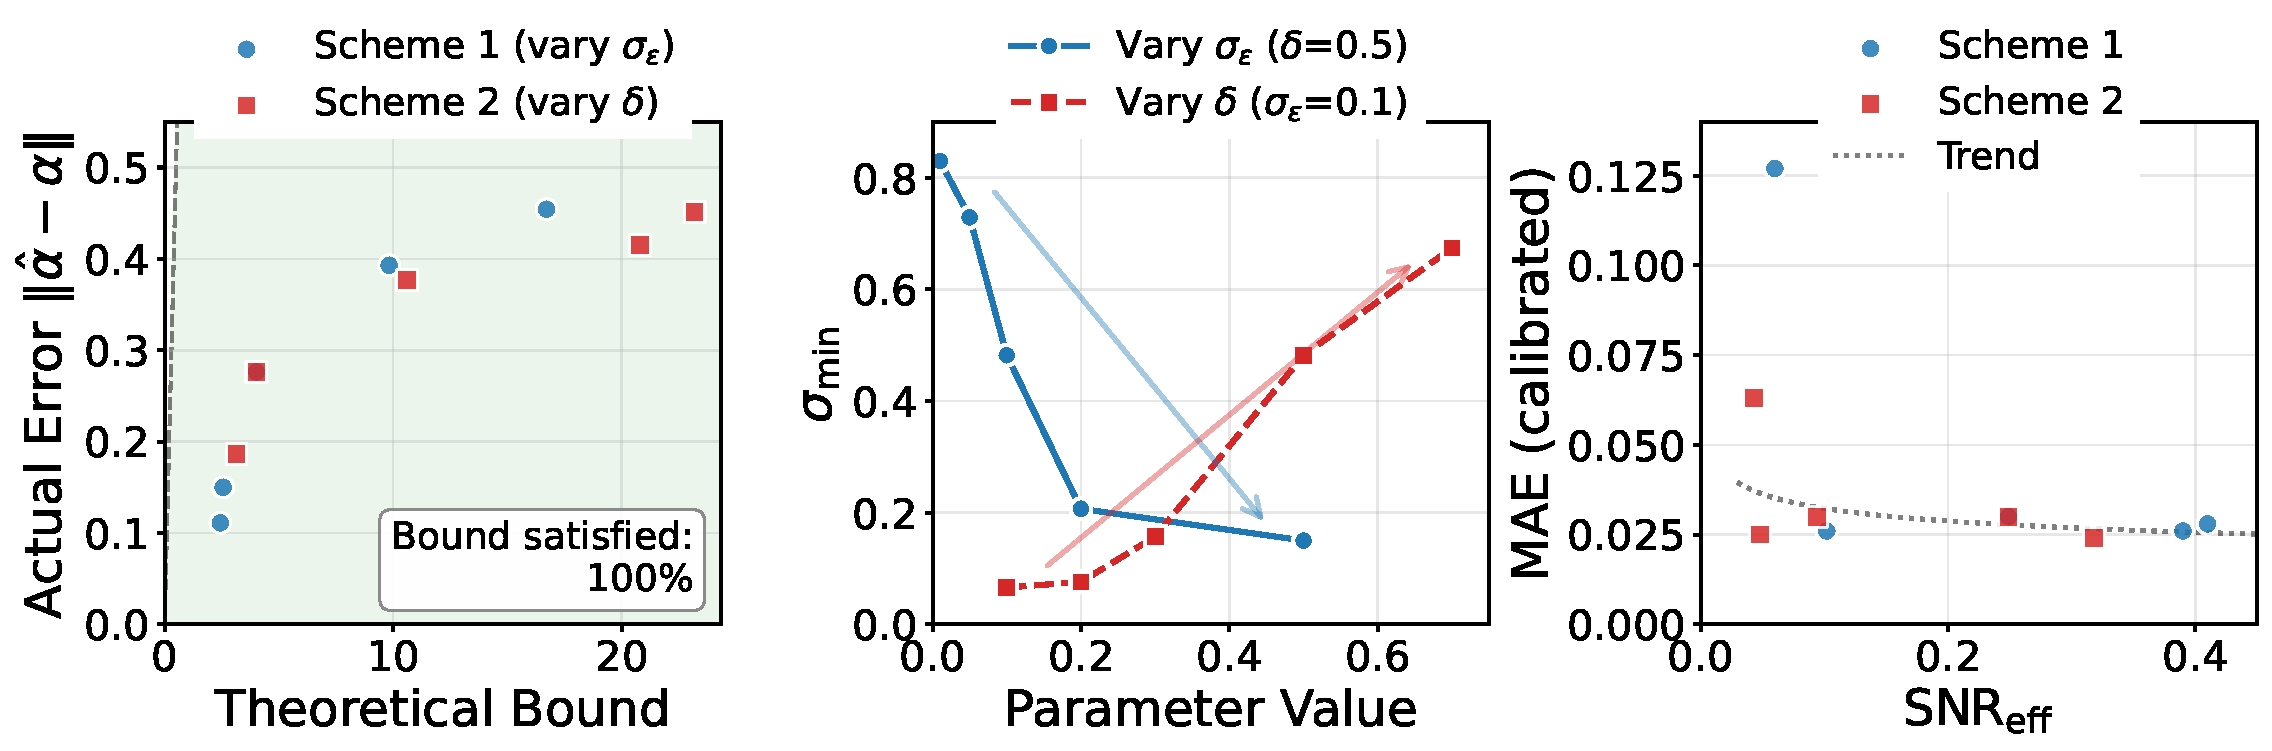
\includegraphics[width=0.62\textwidth]{figures/theory_validation_3panel.pdf}
  \caption{Left: recovery of $\va(t)$ with $K_{\text{active}}=3$ (domains 0, 2, 4), Corr.\ $0.99$ after calibration. Right: empirical check of Theorem~\ref{thm:recovery}, with recovery error against the theoretical bound (all points below $y=x$), $\smin$ under varying noise and perturbation, and MAE against the effective SNR.}
  \label{fig:synthetic}
\end{figure*}

\begin{figure}[!t]
  \centering
  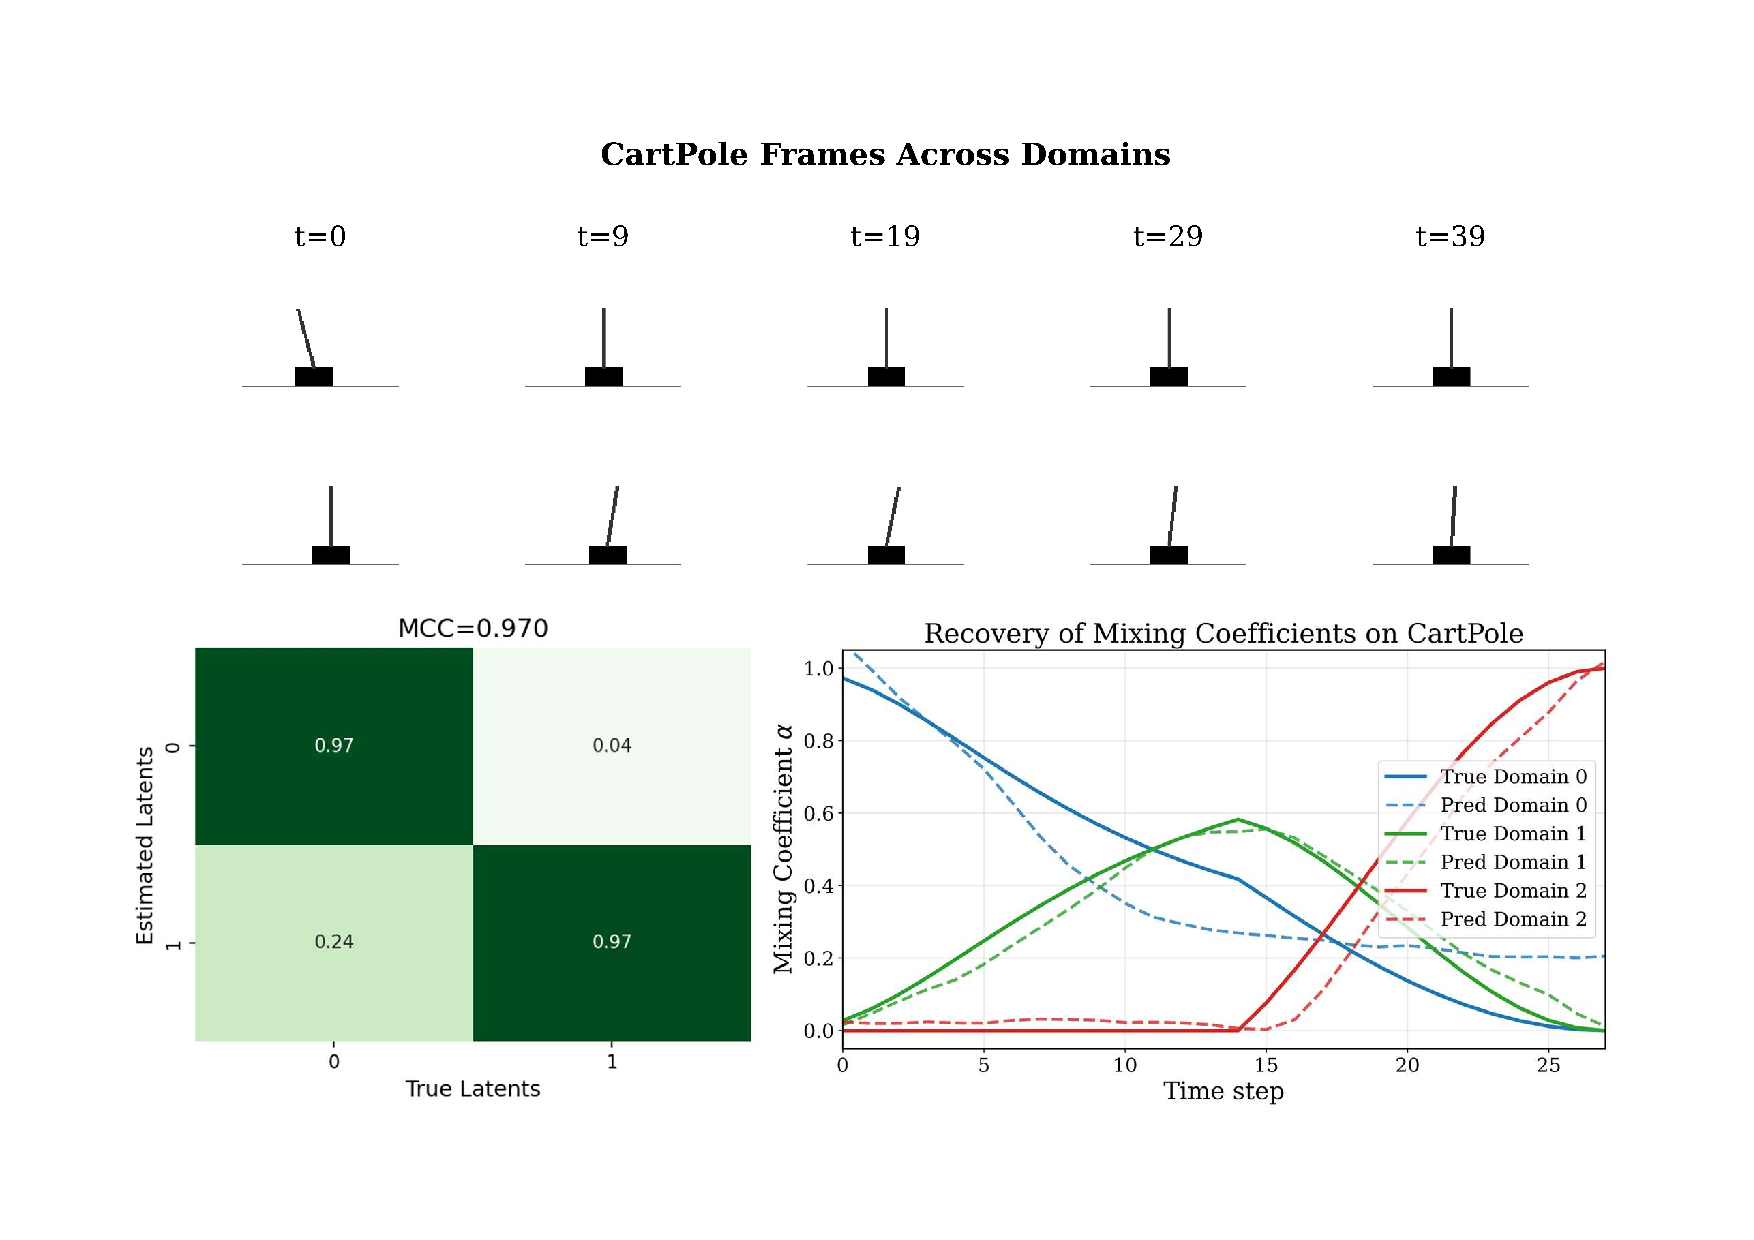
\includegraphics[width=\columnwidth]{figures/cartpole_combined.pdf}
  \caption{Modified CartPole. Top: frames from different domains. Bottom left: correlation matrix of recovered latents (MCC $0.970$). Bottom right: recovered mixing coefficients (Corr.\ $0.95$).}
  \label{fig:cartpole}
\end{figure}

%----------------------------------------------------------------------

\paragraph{Generative model.}
Let $\vz_t\in\mathbb{R}^d$ be latent causal variables and $\vx_t\in\mathbb{R}^p$ the observation,
\begin{equation}
\vz_t = \sigma\big(W(t)\,\vz_{t-1}\big) + \boldsymbol{\epsilon}_t,\qquad \vx_t = g(\vz_t),
\label{eq:model}
\end{equation}
where $g$ is an invertible nonlinear mixing function, $\sigma$ a component-wise activation (e.g.\ LeakyReLU) and $\boldsymbol{\epsilon}_t$ independent noise. Prior work assumes $W(t)\in\{W^{(0)},\dots,W^{(K-1)}\}$. We instead let
\begin{equation}
W(t)=\sum_{k=0}^{K-1}\alpha_k(t)\,W^{(k)},\qquad \va(t)\in\Delta^{K-1},
\label{eq:mix}
\end{equation}
so the causal graph moves continuously inside the simplex spanned by $K$ atomic mechanisms.

\begin{assumption}[Distinguishable mechanisms]
\label{ass:indep}
No $W^{(k)}$ is a convex combination of the others. Concretely, for each latent dimension $i$ the rows $\{(W^{(k)}-W^{(0)})_{i,:}\}_{k=1}^{K-1}$ are linearly independent, which implies the capacity limit $K\le d+1$.
\end{assumption}

\paragraph{Task.}
During training we observe labeled trajectories from the $K$ pure domains ($\va$ one-hot). At test time we observe an unlabeled trajectory $\vx_{1:T}$ whose $\va(t)$ varies smoothly, with neither latents nor labels available. The goal is (i) latents $\hat\vz_t$ identifiable up to permutation and component-wise transformation, and (ii) the trajectory $\{\va(t)\}_{t=1}^T$.

\paragraph{Identifiability results.}
\begin{theorem}[Latent variables]
\label{thm:latent}
If $g$ is invertible and $p(z_{i,t}\mid\vz_{t-1})$ varies sufficiently across the $K$ domains, any $\hat\vz_t$ satisfying the conditional-independence constraints obeys $\hat z_i=h_i(z_{\pi(i)})$ for a permutation $\pi$ and strictly monotone $h_i$.
\end{theorem}
This builds on TDRL~\citep{yaoTemporallyDisentangledRepresentation2022}, which needs an abstract ``sufficient variability'' condition. We show that Assumption~\ref{ass:indep} implies it. Under Gaussian noise,
\begin{equation*}
\frac{\partial^2\log p(z_{i,t}\mid\vz_{t-1},k)}{\partial z_{i,t}\,\partial\vz_{t-1}}=\frac{\sigma'([W^{(k)}\vz_{t-1}]_i)}{\sigma_i^2}\,(W^{(k)})_{i,:}^\top,
\end{equation*}
so cross-domain differences are, to first order, proportional to the rows of $W^{(k)}-W^{(0)}$ and inherit their linear independence when $\sigma'\neq0$.

Let $\hat\vmu^{(k)}$ be the conditional mean of $\hat\vz_t$ under domain $k$, and $\hat B=[\hat\vmu^{(1)}-\hat\vmu^{(0)},\dots,\hat\vmu^{(K-1)}-\hat\vmu^{(0)}]$ with smallest singular value $\smin>0$.
\begin{theorem}[Pointwise recovery]
\label{thm:recovery}
Under Theorem~\ref{thm:latent}, $\hat\va(t)=\hat B^\dagger(\hat\vz_t-\hat\vmu^{(0)})$ satisfies
\begin{equation*}
\|\hat\va(t)-\va(t)\|\le\frac{1}{\smin}\big(\|\hat{\boldsymbol\epsilon}_t\|+\dapx\big),\qquad \dapx=O(\epsilon^2),
\end{equation*}
where $\epsilon=\max_k\|W^{(k)}-W^{(0)}\|$.
\end{theorem}
\noindent\emph{Proof sketch.} By Theorem~\ref{thm:latent}, $\hat\vz=P\,h(\vz)$. Expanding $h$ around $\vmu^{(0)}$ gives $\hat B=PDB$ with $D=\mathrm{diag}(h_i'(\mu_i^{(0)}))$ invertible, so $\hat B$ has full column rank and $\hat B^\dagger\hat B=I$. Writing $\hat\vz_t-\hat\vmu^{(0)}=\hat B\va+r(\va)+\hat{\boldsymbol\epsilon}_t$ with residual $\|r\|\le\dapx$, we get $\hat\va-\va=\hat B^\dagger(r+\hat{\boldsymbol\epsilon}_t)$, and $\|\hat B^\dagger\|=1/\smin$. A second-order Taylor expansion of $f$ in $W$ and of $h$ gives $\dapx=O(\epsilon^2)$. \hfill$\square$

The bound also predicts a \emph{geometric bottleneck}. As $K$ approaches $d+1$ the basis columns become nearly collinear, $\smin$ shrinks, and recovering $\va$ degrades even when every atomic mechanism is learned correctly.

\paragraph{Method (TRACE).}
\begin{figure}[t]
  \centering
  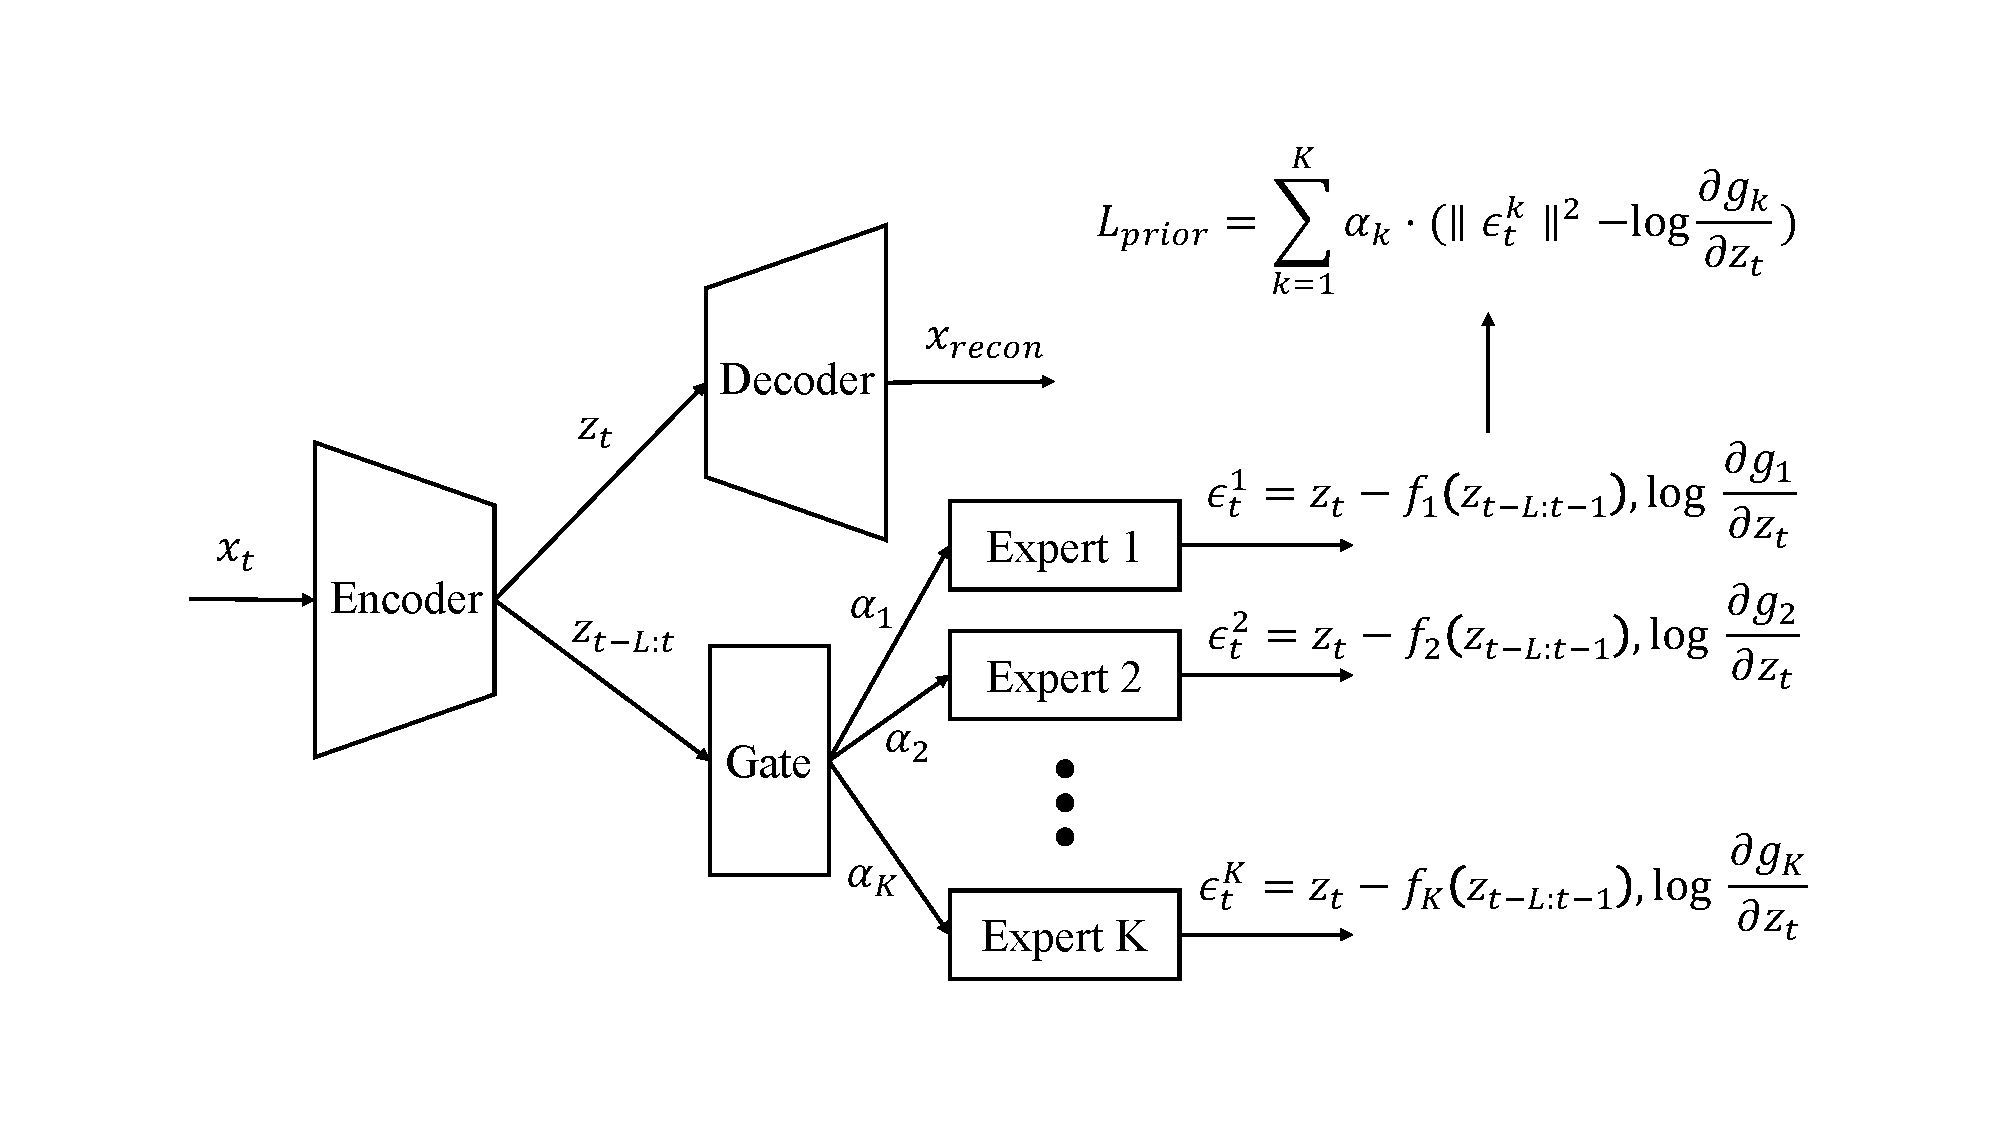
\includegraphics[width=\columnwidth]{figures/TRACE_structure.pdf}
  \caption{TRACE. Stage~1 trains a shared encoder with one-hot gating to domain-specific experts. Stage~2 recovers $\va$ by least-squares projection.}
  \label{fig:arch}
\end{figure}
TRACE has two stages (Figure~\ref{fig:arch}). \textbf{Stage~1} extends a sequential VAE~\citep{kingma2013auto} with an MoE prior. A shared encoder maps $(\vx_t,\vx_{t-L:t-1})$ to a Gaussian posterior, reflecting that the causal variables are shared while their relations change. Expert $k$ is a normalizing flow~\citep{papamakarios2017masked} that maps $\vz_t$ to independent noise given its history, giving the transition prior $p_k(\vz_t\mid\vz_{t-L:t-1})$. One-hot gating routes each training sample to its domain's expert, and we maximize $\mathbb{E}_q[\log p(\vx_t\mid\vz_t)+\log p_k(\vz_t\mid\vz_{t-L:t-1})-\log q(\vz_t\mid\vx_t)]$. \textbf{Stage~2} computes $\hat\vmu^{(k)}$ on validation data of each domain, forms $\hat B$, encodes a test observation by its posterior mean, and applies $\hat\va(t)=\mathrm{Proj}_{\Delta^{K-1}}(\hat B^\dagger(\vz_t-\hat\vmu^{(0)}))$ followed by a moving average with window $2w+1$. No transition data are needed for training, so the method generalizes to intermediate states never observed.

%----------------------------------------------------------------------
\section{Data}
%----------------------------------------------------------------------

\paragraph{Synthetic dynamical system.}
$d=8$ latents with second-order dynamics
\begin{equation*}
\vz_t=\sigma\big(\sigma(\vz_{t-1}W^{(k)})+\sigma(\vz_{t-2}W_{\text{lag2}})\big)+\boldsymbol\epsilon_t,
\end{equation*}
LeakyReLU slope $0.2$ and $\boldsymbol\epsilon_t\sim\mathcal{N}(0,0.1^2I)$. We build $K=5$ atomic mechanisms $W^{(k)}=W_{\text{base}}+\delta W^{(k)}$, where each $\delta W^{(k)}$ modifies one distinct off-diagonal edge, which satisfies Assumption~\ref{ass:indep}. Observations $\vx_t\in\mathbb{R}^{16}$ come from an invertible orthogonal MLP. Training uses 40,000 pure-domain trajectories per domain (200,000 total) of length 50. Test trajectories mix $K_{\text{active}}=3$ domains (e.g.\ $0\to2\to4$) with linear or sinusoidal schedules, so ground-truth $\va(t)$ is known.

\paragraph{Modified CartPole.}
A semi-synthetic system with latent state $(x,v,\theta,\omega)$ rendered as $128\times128$ grayscale frames. Five domains each strengthen one causal edge (e.g.\ $v\to\theta$, $\theta\to\omega$), with constant noise variance across domains. This is a setting where NCTRL's identifiability conditions fail but ours hold. We use 1,000 trajectories of length 100 per domain.

\paragraph{Real-world data.}
\emph{UAVDT}~\citep{Uavdt} provides UAV traffic video with annotated vehicle boxes. We extract turning trajectories at intersections (length $\ge20$ frames, direction change $\ge60^\circ$) and train on straight horizontal and vertical motion as the two atomic mechanisms. \emph{CMU Motion Capture} provides 31-joint skeletons at 120\,Hz. We use walk-to-run trials from six subjects (over 1,000 transition frames, $p=188$ features from joint positions, velocities and hip statistics) and train on pure walking and running. Neither dataset has ground-truth $\va(t)$, so we evaluate against physically motivated proxies (velocity direction for vehicles, normalized hip speed for gait).

%----------------------------------------------------------------------
\section{What We Have Done So Far}

\paragraph{Completed work.}
\begin{enumerate}
\item \textbf{Problem formulation.} Continuous mechanisms as convex combinations of atomic mechanisms (Eqs.~\ref{eq:model}--\ref{eq:mix}), with the distinguishability assumption and its capacity limit $K\le d+1$.
\item \textbf{Theory.} Proofs of latent identifiability (Theorem~\ref{thm:latent}), of the bridge from Assumption~\ref{ass:indep} to sufficient variability, of pointwise recovery of $\va(t)$ (Theorem~\ref{thm:recovery}) and of $\dapx=O(\epsilon^2)$.
\item \textbf{Implementation.} The full TRACE pipeline (Stage~1 MoE sequential VAE and Stage~2 least-squares solver), the data generators for the synthetic system and modified CartPole, and the six baselines.
\item \textbf{Experiments.} Synthetic comparison with baselines, empirical validation of Theorem~\ref{thm:recovery}, and CartPole from pixels.
\end{enumerate}

\paragraph{Implementation details.}
The model is implemented in PyTorch. For synthetic data the encoder and decoder are 3-layer MLPs (hidden size 128), $d=8$, lag $L=2$, and each expert is a normalizing-flow transition prior. We train with Adam (learning rate $5\times10^{-4}$, batch size 64, 100 epochs) with KL weight $\beta=2\times10^{-3}$ and prior weight $\gamma=2\times10^{-2}$. For CartPole the encoder is a CNN (three stride-2 convolutions with 32, 64 and 128 channels followed by FC 256 and FC 4), trained for 200 epochs. Synthetic training takes 6--8 hours on one A100 and CartPole 15--20 hours on two A100s. At test time we use window $w=5$ and two-point scale calibration from the trajectory endpoints.
%----------------------------------------------------------------------

\paragraph{Metrics and baselines.} Latent identifiability is measured by the mean correlation coefficient (MCC)~\citep{hyvarinen2016unsupervised}, and trajectory recovery by the Pearson correlation between true and recovered $\va(t)$ (Corr.). We compare with NCTRL~\citep{song2023temporally} (hard and soft gating), TDRL~\citep{yaoTemporallyDisentangledRepresentation2022}, LEAP~\citep{yao2021learning}, iVAE~\citep{khemakhem2020variational} and PCL~\citep{hyvarinen2017nonlinear}. All baselines assume discrete mechanisms.

\begin{table}[t]
\caption{Synthetic data. MCC is computed on pure-domain test data, Corr.\ on continuous transitions. NA means the method needs discrete labels and cannot output weights during transitions.}
\label{tab:synthetic}
\centering
\small
\begin{tabular}{lcc}
\toprule
Method & Weight Corr.\ $\uparrow$ & Latent MCC $\uparrow$ \\
\midrule
NCTRL (hard) & 0.67 $\pm$ 0.03 & 0.90 $\pm$ 0.09 \\
NCTRL (soft) & 0.72 $\pm$ 0.01 & 0.90 $\pm$ 0.09 \\
TDRL & NA & 0.89 $\pm$ 0.03 \\
LEAP & NA & 0.66 $\pm$ 0.05 \\
iVAE & NA & 0.53 $\pm$ 0.02 \\
PCL & NA & 0.59 $\pm$ 0.04 \\
\textbf{TRACE} & \textbf{0.94 $\pm$ 0.05} & \textbf{0.96 $\pm$ 0.03} \\
\bottomrule
\end{tabular}
\end{table}

\paragraph{Synthetic results.}
Table~\ref{tab:synthetic} shows that TRACE reaches the highest trajectory correlation ($0.94$ versus $0.72$ for NCTRL-soft) and the highest latent MCC ($0.96$). Figure~\ref{fig:synthetic} (left) shows a three-domain transition. After two-point scale calibration the recovered trajectory tracks both the sequential activation and the timing of the intermediate peak (Corr.\ $0.99$).



\begin{table}[t]
\caption{Checking the predictions of Theorem~\ref{thm:recovery}. MAE before (raw) and after (cal) scale calibration; $\mathrm{SNR}_{\text{eff}}=\smin/(\bar\epsilon+\dapx)$.}
\label{tab:snr}
\centering
\footnotesize
\setlength{\tabcolsep}{4pt}
\begin{tabular}{lccccc}
\toprule
\multicolumn{6}{c}{Vary noise $\sigma_\epsilon$ ($\|W^{(k)}-W^{(0)}\|_F=0.5$)}\\
\midrule
$\sigma_\epsilon$ & 0.01 & 0.05 & 0.10 & 0.20 & 0.50 \\
MCC & 0.996 & 0.994 & 0.984 & 0.849 & 0.703 \\
Corr. & 0.998 & 0.998 & 0.998 & 0.996 & 0.854 \\
MAE\textsubscript{raw} & 0.077 & 0.106 & 0.254 & 0.278 & 0.321 \\
MAE\textsubscript{cal} & 0.028 & 0.026 & 0.030 & 0.026 & 0.127 \\
\midrule
\multicolumn{6}{c}{Vary perturbation ($\sigma_\epsilon=0.1$)}\\
\midrule
$\|W^{(k)}-W^{(0)}\|_F$ & 0.1 & 0.2 & 0.3 & 0.5 & 0.7 \\
MCC & 0.934 & 0.953 & 0.970 & 0.984 & 0.990 \\
Corr. & 0.972 & 0.996 & 0.997 & 0.998 & 0.998 \\
MAE\textsubscript{raw} & 0.319 & 0.292 & 0.266 & 0.254 & 0.194 \\
MAE\textsubscript{cal} & 0.063 & 0.025 & 0.030 & 0.030 & 0.024 \\
\bottomrule
\end{tabular}
\end{table}

\paragraph{Validating the theory.}
We vary the noise level and the perturbation size (Table~\ref{tab:snr}). Three observations match the theory. Corr.\ stays above $0.97$ even when MCC degrades, so the trajectory shape is preserved. Calibration reduces MAE by $3$--$10\times$, consistent with the bias term $\hat B^\dagger r(\va)$ acting as a near-linear distortion. Both MCC and MAE improve as the perturbation grows, as predicted by the $1/\smin$ dependence. Figure~\ref{fig:synthetic} (right) confirms that every recovery error lies below the bound of Theorem~\ref{thm:recovery}.

\paragraph{CartPole from pixels.}

Figure~\ref{fig:cartpole} shows that TRACE recovers the observable latents $(x,\theta)$ from $128\times128$ frames with MCC $0.970$ and recovers the three-domain trajectory with Corr.\ $0.95$, so the framework extends from vectors to images.

%----------------------------------------------------------------------
\section{What Remains to Be Done}
%----------------------------------------------------------------------

\begin{enumerate}
\item \textbf{Trajectory-level theory (by Nov 20).} Theorem~\ref{thm:recovery} treats each time step independently, so its bound does not improve with $T$. We will exploit the smoothness of $\va(t)$ (bounded total variation) through a regularized estimator and derive a finite-sample error rate in $T$, with complete proofs.
\item \textbf{Real-world experiments (by Nov 15).} Finish the UAVDT vehicle-turning and CMU walk-to-run experiments, comparing TRACE with NCTRL against the proxy trajectories.
\item \textbf{Capacity ablation (by Nov 22).} Train with $K_{\text{total}}=10$ and evaluate $K_{\text{active}}\in\{2,\dots,7\}$ on sequential, overlapping and oscillating schedules, reporting recovery of both $\va(t)$ and $W(t)$, to test the geometric bottleneck predicted by Theorem~\ref{thm:recovery}.
\item \textbf{Robustness (by Nov 25).} Smoothing window size, a Kolmogorov--Smirnov test of the convex-interpolation assumption, and out-of-distribution transitions.
\item \textbf{Deliverables.} Final presentation (mid November) and the 8--10 page final report with full proofs (December 1).
\end{enumerate}

\section*{Team Contributions}
Shicheng Fan and Jie Yang ran the experiments. All three members discussed the theoretical framework and the proofs together. Honghui Bao wrote this report.

\section*{Code Availability}
Code, data generators and reports are maintained at \url{https://github.com/HonghuiBao2000/cs412-trace}.

\bibliographystyle{ACM-Reference-Format}
\bibliography{references}

\end{document}
